\documentclass{beamer}
\usefonttheme[onlymath]{serif}

\usepackage{amsfonts}

% Code Block Setting
\usepackage{listings}
\lstset{language=C,
numberstyle=\footnotesize,
basicstyle=\ttfamily\footnotesize,
numbers=left,
stepnumber=1,
frame=shadowbox,
breaklines=true}

\usetheme{Warsaw}
% \usecolortheme{dove}

% Add frame number and total frame number in footline
\defbeamertemplate*{footline}{shadow theme}{%
    \leavevmode%
    \hbox{\begin{beamercolorbox}[wd=.5\paperwidth,ht=2.5ex,dp=1.125ex,leftskip=.3cm plus1fil,rightskip=.3cm]{author in head/foot}%
            \usebeamerfont{author in head/foot}\hfill\insertshortauthor
        \end{beamercolorbox}%
        \begin{beamercolorbox}[wd=.4\paperwidth,ht=2.5ex,dp=1.125ex,leftskip=.3cm,rightskip=.3cm plus1fil]{title in head/foot}%
            \usebeamerfont{title in head/foot}\insertshorttitle\hfill%
        \end{beamercolorbox}%
        \begin{beamercolorbox}[wd=.1\paperwidth,ht=2.5ex,dp=1.125ex,leftskip=.3cm,rightskip=.3cm plus1fil]{title in head/foot}%
            \hfill\insertframenumber\,/\,\inserttotalframenumber
    \end{beamercolorbox}}%
    \vskip0pt%
}

% Tikz related
\usepackage{tikz}
\usetikzlibrary{fit}
\usetikzlibrary{calc}
\usetikzlibrary{positioning}

% Number the figures
\setbeamertemplate{caption}[numbered]

% Add outline page at begining of each section
\AtBeginSection[]
{
    \begin{frame}<beamer>
        \frametitle{Outline}
        \tableofcontents[currentsection, hideallsubsections]
    \end{frame}
}

%%%%%%%%%%%%%%%%%%%%%%%%%%%%%%%%%%%%%%%%%%%%%

\title{swDNN:A Library for Accelerating Deep Learning Applications on Sunway TaihuLight}
\author{
    Jiarui Fang,
	Haohuan Fu,
    Wenlai Zhao,
    Bingwei Chen,
    Weijie Zheng,
    Guangwen Yang,\\
}
\institute{
    \inst{1} Department of Computer Science and Technology, Tsinghua University
	\inst{2} Ministry of Education Key Lab. for Earth System Modeling, Department of Earth System Science, Tsinghua University
	\inst{3} National Supercomputing Center in Wuxi
}
\date{
    \tiny{2017 IEEE International Parallel and Distributed Processing Symposium}\\
    \tiny{Presented by Ching-Yuan, Tsai}
}

\begin{document}
\begin{frame}
    \titlepage
\end{frame}
\section{Introduction}

\subsection{SIMD}
\begin{frame}
    \frametitle{SIMD}
	\begin{itemize}
		\item Single instruction multiple data
		\item without threads support
	\end{itemize}
\end{frame}


\subsection{VPU}
\begin{frame}
    \frametitle{VPU}
	\begin{itemize}
		\item Vector processing units 
		\item combine itstructions as vector	
	    \begin{figure}
			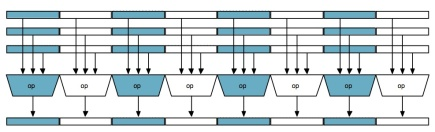
\includegraphics[scale=0.5]{figure/vpu.jpg}
		\end{figure}
	\end{itemize}
\end{frame}


\section{Architecture}

\subsection{Architecture}
\begin{frame}
    \frametitle{Architecture}
	\begin{figure}
		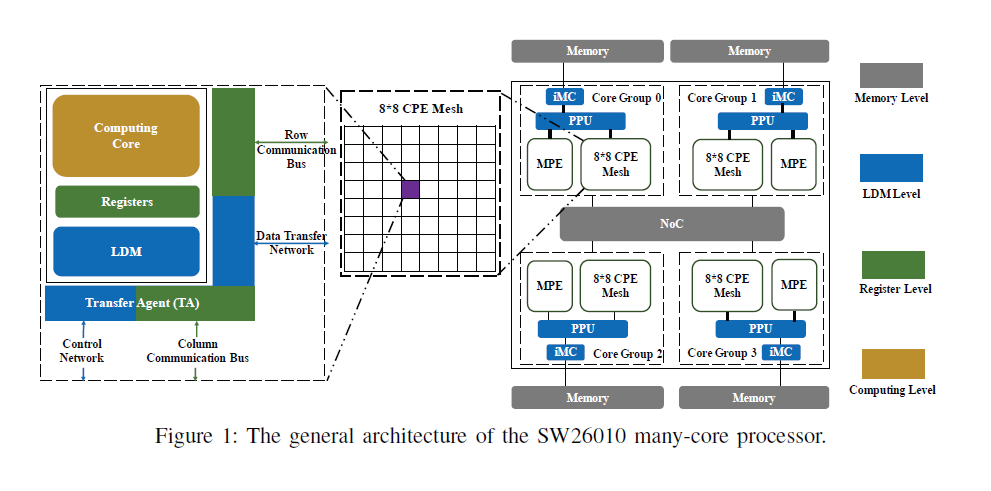
\includegraphics[scale=0.4]{figure/archi.PNG}
	\end{figure} 
\end{frame}

\subsection{Unique features}
\begin{frame}
    \frametitle{Unique features}
	\begin{itemize}
		\item Each CG has an MPE.
		\item Users can explicitly set the sizeof each CG's private memory space, and the size of shared memory space.  
		\item Support a 64kb user-controlled fast buffer for each computing cores. 
		\item Rigister communication between computing cores.
		\item Each computing core consists of two execution pipelines.  
	\end{itemize} 
\end{frame}

\subsection{Challenges}
\begin{frame}
    \frametitle{Challenges}
	\begin{itemize}
		\item Low memory bandwidth. 
		\begin{itemize}
			\item SW26010:36 GB/s for each CG, 144 GB/S for entire processor.  
			\item NVIDIA K80GPU: 480 GB/S for entire processor. 
		\end{itemize}
		\item CPEs do not have a shared buffer to rely on a fine-grained data sharing scheme. 
	\end{itemize}
\end{frame}

	


%\section{Performance model}

\subsection{Performance model}
\begin{frame}
    \frametitle{Performance model}
	\begin{itemize}
		\item Two diffenent scenarios
		\begin{itemize}
			\item CPEs directly access global memory.(from global mem to register)  
			\item Three-level memory hierarchy.(REG-LDM-MEM)
		\end{itemize}
	\end{itemize} 
\end{frame}

\begin{frame}
	\frametitle{Performance model}
	\begin{figure}
		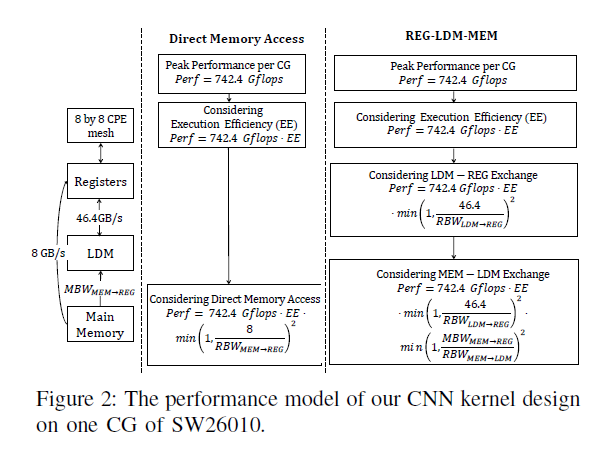
\includegraphics[scale=0.5]{figure/performancemodel.PNG}
	\end{figure}
\end{frame}

\begin{frame}
	\frametitle{$MBW_{MEM to LDM}$}
	\begin{figure}
		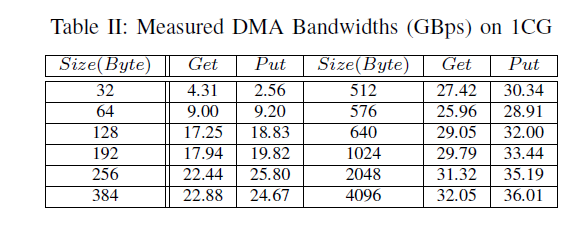
\includegraphics[scale=0.5]{figure/performancetable.PNG}
	\end{figure}
\end{frame}


	


\section{Register Communication}

\subsection{Register Communication}
\begin{frame}
    \frametitle{Register Communication}
	\begin{itemize}
		\item Motivation
		\begin{itemize}
			\item Fine-grained.
			\item No shared memory in a CG.
		\end{itemize}
		\item Architecture
		\begin{itemize}
			\item 8 row communication buses.
			\item 8 col communication buses.
			\item Broadcast. 
		\end{itemize}
	\end{itemize} 
\end{frame}
\subsection{Example}
\begin{frame}
	\frametitle{$W*D_{i}=D_{o}$}
	\begin{figure}
		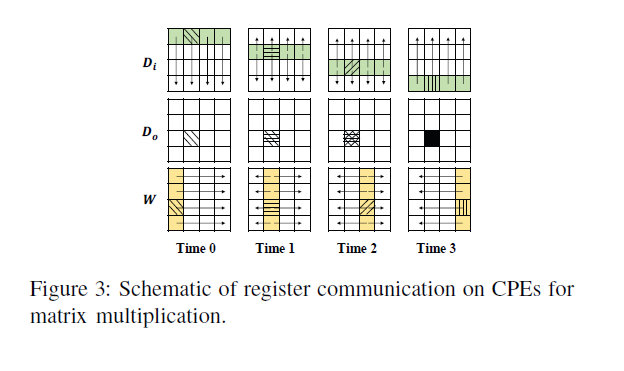
\includegraphics[scale=0.5]{figure/broadcast.PNG}
	\end{figure}
\end{frame}



	


\section{Instruction Pipelines}

\subsection{P1 and P0}
\begin{frame}
    \frametitle{P1 and P0}
	\begin{itemize}
		\item Each CPE consists of two execution pipelines.
		\begin{itemize}
			\item P0 : floating-pointer, vector operations. 
			\item P1 : Control transfer, load/store and register communication operations.
		\end{itemize}
		\item The two execution pipelines share an Instruction Decoder and an instruction queue.
		\item In each cycle, two instructions in the front of the queue are issued into two pipelines.
	\end{itemize} 
\end{frame}
\subsection{Instructions scheduling rules}
\begin{frame}
	\frametitle{Instructions scheduling rules}
	\begin{itemize}
		\item Both instructions have no conflicts with the unifinished instructions issued before. 
		\item The two insturctions have no RAW or WAW conflicts.
		\item The two instructions can be handled by two execution pipelines separately.  
	\end{itemize}
\end{frame}



	


\section{Experiment}

\subsection{Sparse Matrices}
\begin{frame}
	\frametitle{Sparse Matrices}
	\begin{figure}
		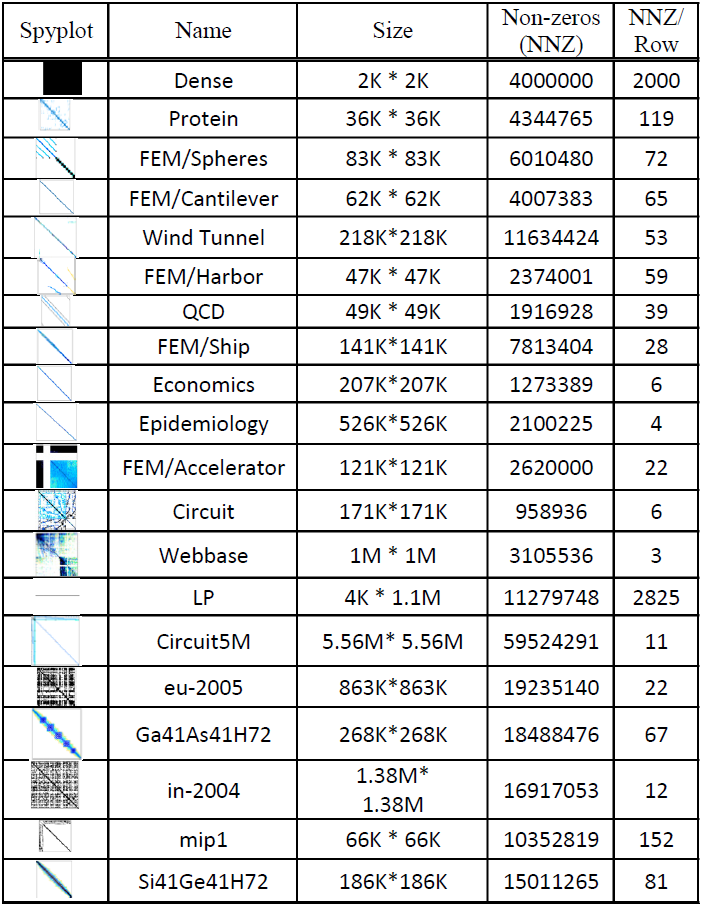
\includegraphics[scale=0.25]{figure/fig5-kindmatrices.png}
	\end{figure}
\end{frame}

\subsection{Memory Footprint}
\begin{frame}
	\frametitle{Memory Footprint}
	\begin{figure}
		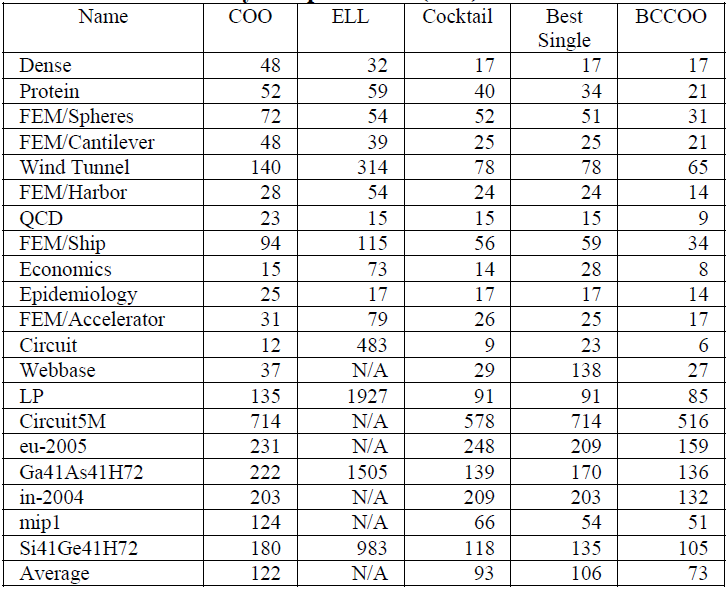
\includegraphics[scale=0.4]{figure/fig6-memoryprint.png}
	\end{figure}
\end{frame}

\subsection{Performance Comparison}
\begin{frame}
	\frametitle{Performance Comparison between Other Algorithms}
	\begin{figure}
		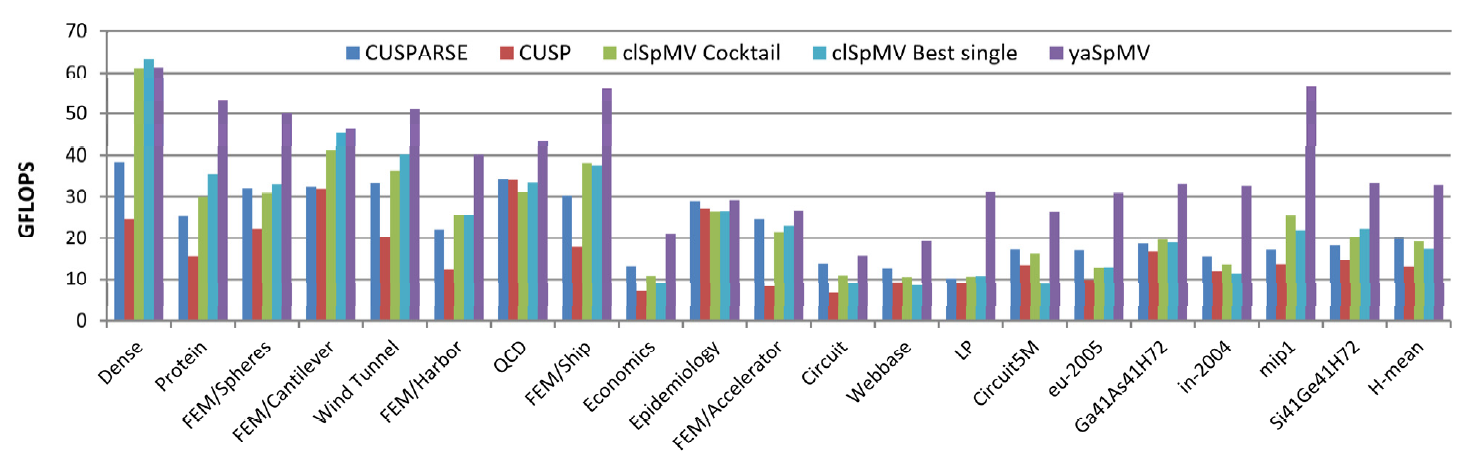
\includegraphics[scale=0.25]{figure/fig7-exp1.png}
	\end{figure}
\end{frame}

\begin{frame}
	\frametitle{Performance Comparison between Different Optimizations}
	\begin{figure}
		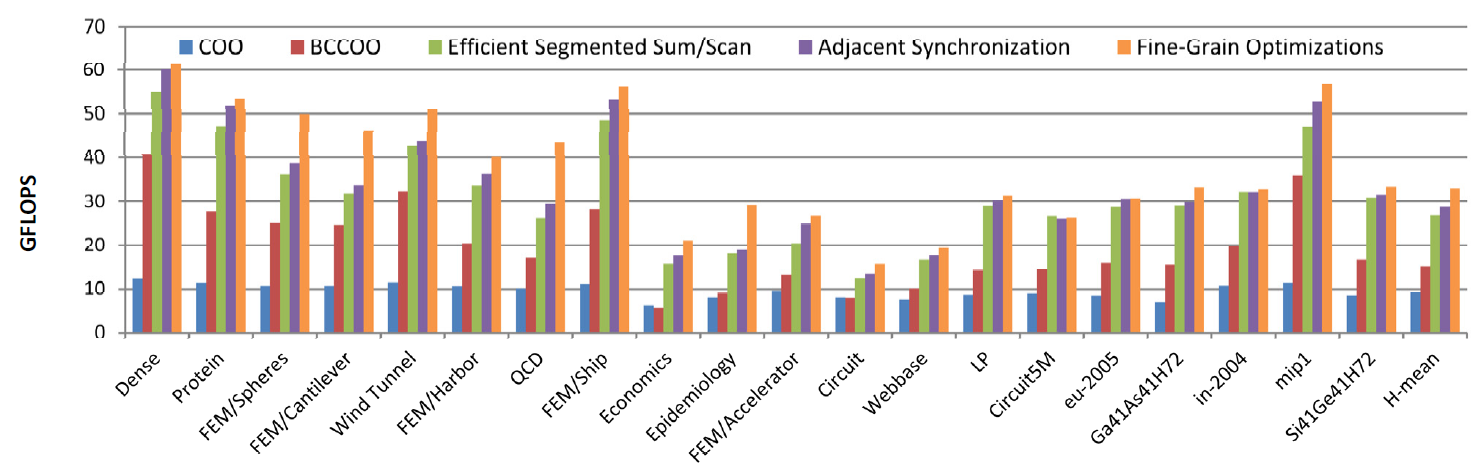
\includegraphics[scale=0.25]{figure/fig8-exp2.png}
	\end{figure}
\end{frame}
\end{document}
